\documentclass[a4paper,french,bookmarks]{article}
\usepackage{./Structure/4PE18TEXTB}

\lstset{language=Caml,keywordstyle={\color{main1}}}

\newcommand{\rouge}{{\color{main9} rouge}}
\newcommand{\rouges}{{\color{main9} rouges}}
\DeclareMathOperator{\etiquettes}{etiquettes}
\newboxans

\begin{document}
\stylizeDoc{Informatique}{Devoir Maison 3}{Implémentation des arbres bicolores en OCaml}

\hfill\\[-35pt]
\begin{center}
    \begin{minipage}{0.8\linewidth}
        \begin{tcolorbox}[
            breakable,
            enhanced,
            interior style      = {left color=main4!15,right color=main2!12},
            borderline north    = {.5pt}{0pt}{main2!10},
            borderline south    = {.5pt}{0pt}{main2!10},
            borderline west     = {.5pt}{0pt}{main2!10},
            borderline east     = {.5pt}{0pt}{main2!10},
            sharp corners       = downhill,
            arc                 = 0 cm,
            boxrule             = 0.5pt,
            drop fuzzy shadow   = black!40!white,
            nobeforeafter,
        ]
        \centering\GillSansMT Les codes écrits ci-dessous sont accessible à l'adresse \textit{\color{main2}\href{https://gitlab.com/-/snippets/2302097}{https://gitlab.com/-/snippets/2302097}}
    \end{tcolorbox}
\end{minipage}
\end{center}

\section{Introduction}

L'objectif de ce sujet est d'obtenir une implémentation complète des arbres \rouge{}-noir fonctionnels en OCaml : test d'appartenance, insertion, et suppression. Pour cela, on va travailler avec le type suivant :

\begin{ocaml}
type 'a rn =
    | V
    | N of 'a rn * 'a * 'a rn (* noeud noir *)
    | R of 'a rn * 'a * 'a rn (* noeud rouge *)
;;
\end{ocaml}
    
Rappelons les contraintes que doit respecter un arbre \rouge{}-noir :

\begin{enumerate}
    \ithand ce doit être un ABR (\ie{} les étiquettes lues dans l'ordre infixe sont strictement croissantes) ;
    
    \ithand un nœud \rouge{} ne peut pas avoir un fils \rouge{} ;
    
    \ithand tous les chemins de la racine à un nœud vide contiennent le même nombre de nœuds noirs ;
    
    \ithand la racine est noire.
\end{enumerate}

On appellera :

\begin{enumerate}
    \ithand \textbf{arbre \rouge{}-noir correct} un arbre vérifiant les 4 conditions ci-dessus ;
    
    \ithand \textbf{sous-arbre \rouge{}-noir correct} un arbre vérifiant les 3 premières conditions (peut être pas la dernière) ;
    
    \ithand \textbf{sous-arbre \rouge{}-noir \textit{presque} correct} un arbre vérifiant les 3 premières conditions, sauf que sa racine peut être \rouge{} et posséder un (ou deux) fils \rouges{}.
\end{enumerate}

Il arrivera souvent que la couleur de la racine n'importe pas. Dans ce cas, plutôt que de faire deux fois la même chose, on pourrait utiliser une fonction construisant un arbre $\left(g, x, d\right)$ dont la racine est de la même couleur que l'arbre de départ.

\begin{enumerate}
    \item Écrire une fonction \camlline{cons : -> 'a rn -> 'a rn -> 'a -> 'a rn -> 'a rn} ayant la spécification suivante :
    %
    \begin{enumerate}
        \itt \textbf{Entrée :} un arbre $t$ non vide, un arbre $g$, une clé $x$, et un arbre $d$ ;
        
        \itt \textbf{Sortie :} un arbre $t'$ tel que $t' =$ \camlline{N(g,x,d)} si la racine de $t$ est noire, et $t' =$ \camlline{R(g,x,d)} si la racine de $t$ est \rouge{}.
    \end{enumerate}
    
    \begin{ocaml}
let cons (t : 'a rn) (g : 'a rn) (x: 'a) (d : 'a rn) : 'a rn = match t with
    | V -> failwith "L'arbre t est vide"
    | N(_, _, _) -> N(g, x, d)
    | R(_, _, _) -> R(g, x, d)
;;
    \end{ocaml}

\end{enumerate}

\section{Insertion}

Le principe est le suivant : on crée une nouvelle feuille \rouge{} avec la clé à insérer, puis on corrige les problèmes en remontant jusqu'à la racine. Dans ce sujet, on ne fera pas explicitement de \textbf{rotations} mais on utilisera la puissance des \textbf{filtrages par motifs}. Avec cette stratégie, on ne violera jamais la condition d'équilibre noir (troisième condition). Le seul problème potentiel sera un nœud \rouge{} $n$ avec un fils \rouge{}, et la résolution de ce problème sera la
responsabilité du père de $n$ (qui est nécessairement noir). Dans les schémas de ce sujet :

\begin{enumerate}
    \ithand les nœuds \rouges{} et les arêtes menant à un nœud \rouges{} sont en \rouge{} et en gras (donc visible avec impression) ;
    
    \ithand les nœuds noirs sont grisés et les arêtes menant à un nœud noirs sont en trait plein et d'épaisseur normale ;
    
    \ithand les arêtes en pointillés mènent à des nœuds de couleur inconnue.
\end{enumerate}

La figure \ref{fig:fig1} résume les 4 cas possibles pour le père de $n$, et comment les résoudre (toujours de la même manière) de façon à obtenir un sous-arbre \rouge{}-noir \textbf{correct} dans lequel les profondeurs noires n'ont pas
été modifiées.

\begin{center}
	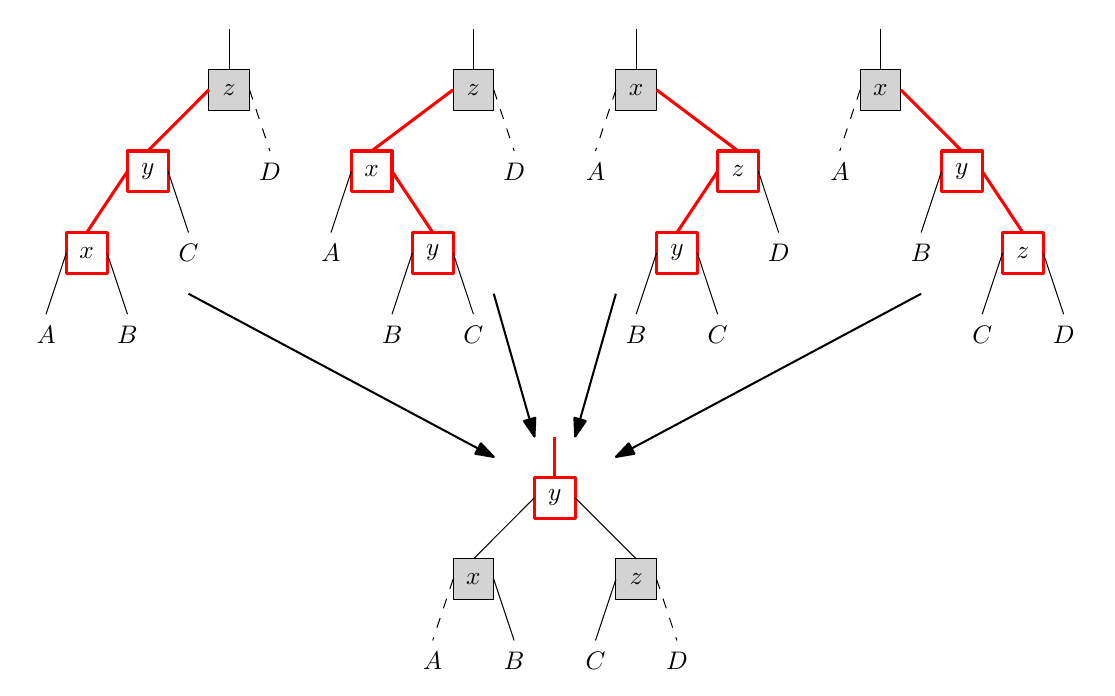
\includegraphics[scale=0.7]{dm3fig/fig1.png}
	\captionof{figure}{Traitement des 4 cas \rouge{}-\rouge{}.}
	\label{fig:fig1}
\end{center}

\begin{enumerate}
    \setcounter{enumi}{1}
    \item Écrire une fonction \camlline{corrige_rouge : 'a rn -> 'a rn} qui prend en entrée un arbre et :
    %
    \begin{enumerate}
        \itt effectue la transformation de la figure \ref{fig:fig1} si c'est nécessaire (racine noire, et un fils \rouge{} qui a un fils \rouge{}) ;
        
        \itt renvoie l'arbre tel quel sinon.
    \end{enumerate}
    %
    Cette fonction renverra un sous-arbre \rouge{}-noir \textbf{presque correct}.
    
    \begin{ocaml}
let corrige_rouge (t : 'a rn) : 'a rn = match t with
    | N(R(R(a, x, b), y, c), z, d) | N(R(a, x, R(b, y, c)), z, d)
    | N(a, x, R(R(b, y, c), z, d)) | N(a, x, R(b, y, R(c, z, d)))
     -> R(N(a, x, b), y, N(c, z, d))
    | _ -> t
;;
    \end{ocaml}
    
    \item Écrire une fonction \camlline{insere_aux : 'a rn -> 'a -> 'a rn} qui prend en entrée un sous-arbre \rouge{}-noir \textbf{correct} et une clé, et renvoie un sous-arbre \rouge{}-noir \textbf{presque correct} dans lequel la clé fournie a été insérée.
    
    \begin{ocaml}
let rec insere_aux (t : 'a rn) (x : 'a) : 'a rn = match t with
    | V -> R(V, x, V)
    | N(g, y, d) -> if x < y then corrige_rouge (N((insere_aux g x), y, d))
     else if x = y then t else corrige_rouge (N(g, y, (insere_aux d x)))
    | R(g, y, d) -> if x < y then corrige_rouge (R((insere_aux g x), y, d))
     else if x = y then t else corrige_rouge (R(g, y, (insere_aux d x)))
;;
    \end{ocaml}
    
    \item Écrire une fonction \camlline{insere : 'a rn -> 'a -> 'a rn} qui prend en entrée un sous-arbre \rouge{}-noir correct et une clé, et renvoie un sous-arbre \rouge{}-noir \textbf{correct} dans lequel la clé fournie a été insérée.
    
    \begin{ocaml}
let insere (t : 'a rn) (x : 'a) : 'a rn = match insere_aux t x with
    | R(g, k, d) -> N(g, k, d)
    | t' -> t'
;;
    \end{ocaml}

\end{enumerate}

\section{Suppression}

Le principe général de la suppression est le suivant :

\begin{enumerate}
    \ithand on commence par rechercher l'élément à supprimer (s'il n'est pas présent, il n'y a rien à faire) ;
    
    \ithand s'il a au plus un fils non vide, on le supprime (en renvoyant son éventuel fils non vide) ;
    
    \ithand sinon, on le remplace par son \textbf{successeur} (le minimum de son fils droit), et on supprime ce successeur ;
    
    \ithand dans les deux cas, on risque d'avoir introduit une violation de la condition d'équilibre noir ;
    
    \ithand on déplace ce problème vers le haut de l'arbre, où on le règle suivant le cas ;

    \ithand en s'occupant de ce problème, on risque de violer la condition \rouge{}-\rouge{}, mais il sera toujours possible de rétablir immédiatement cette propriété.
\end{enumerate}

\subsection{Cas de base pour la suppression}

Il y a 4 cas de base où l'on peut directement supprimer un élément $x$, suivant que le nœud à supprimer est rouge ou noir et que son fils gauche ou droit est vide. On a représenté en figure \ref{fig:fig2} les deux cas correspondant à un fils gauche vide.

\begin{center}
	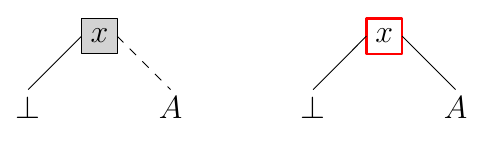
\includegraphics[scale=0.7]{dm3fig/fig2.png}
	\captionof{figure}{Cas de base pour la suppression.}
	\label{fig:fig2}
\end{center}

\begin{enumerate}
    \setcounter{enumi}{4}
      
    \item Indiquer dans les deux cas le résultat de la suppression, en précisant si la profondeur noire a été modifiée ou non (et si oui, comment).
      
    \boxans{
        \begin{minipage}[t]{0.45\linewidth}
            Dans le cas de gauche, on obtient :
            
            \begin{center}
                \begin{tikzpicture}
                    \draw[] (-2.3, 0.7) -- (-2.3, 0);
                    \draw[] (-2.3, 0) -- (-3, -0.7);
                    \draw[main9, thick] (-2.3, 0) -- (-1.6, -0.7);
                    \node at (-2.3,0) [rectangle,draw,fill=black!12, inner sep=5pt] {$x\vphantom{A}$};
                    \node at (-3,-1) [rectangle,fill=white, inner sep=5pt] {$\bot\vphantom{A}$};
                    \node at (-1.6,-1) [rectangle,fill=white,draw=main9, thick, inner sep=5pt] {$A$};
                    
                    \draw[->, thick] (-1, 0) -- (0, 0);;
                    
                    \draw[main9, thick] (1, 0.7) -- (1, 0);
                    \node at (1,0) [rectangle,draw=main9,thick,fill=white, inner sep=5pt] {$A$};
                \end{tikzpicture}
            \end{center}
            
            Puisque le fils gauche de $x$ est nœud vide, le chemin de la racine à ce nœud contient autant de nœuds noirs que le chemin de la racine aux sous-nœuds vide de $A$. Ainsi, $A$ est forcément \rouge{} avant la suppression, puisqu'il est au même \guill{niveau} que le nœud vide. La profondeur noire est donc réduite de 1 lors de la suppression de $x$.
        \end{minipage}
        %
        \hfill
        %
        \begin{minipage}[t]{0.45\linewidth}
            Dans le cas de droite, on obtient :
            
            \begin{center}
                \begin{tikzpicture}
                    \draw[main9, thick] (-2.3, 0.7) -- (-2.3, 0);
                    \draw[] (-2.3, 0) -- (-3, -0.7);
                    \draw[] (-2.3, 0) -- (-1.6, -0.7);
                    \node at (-2.3,0) [rectangle,draw=main9,thick, fill=white, inner sep=5pt] {$x\vphantom{A}$};
                    \node at (-3,-1) [rectangle,fill=white, inner sep=5pt] {$\bot\vphantom{A}$};
                    \node at (-1.6,-1) [rectangle,fill=white, inner sep=5pt] {$A = \bot$};
                    
                    \draw[->, thick] (-1, 0) -- (0, 0);;
                    
                    \draw[] (1, 0.7) -- (1, 0);
                    \node at (1,0) [rectangle,fill=white, inner sep=5pt] {$\bot$};
                \end{tikzpicture}
            \end{center}
            
            On a ici supprimé un nœud \rouge{}, son enfant $A$ est donc nécessairement noir ou vide. Si $A$ n'est pas vide, il y a un plus grand nombre de nœuds noirs entre la racine et les sous-nœuds vides de $A$ qu'entre la racine et le fils vide $\bot$ de $x$, ce qui n'est pas possible. Donc $A = \bot$. La profondeur noire n'est alors pas changée.
        \end{minipage}
    }
\end{enumerate}

\subsection{Suppression du minimum}

On veut écrire une fonction \camlline{supprime_min : 'a rn -> ('a rn * bool)} ayant la spécification suivante :

\begin{enumerate}
    \itt \textbf{Entrée :} un sous-arbre \rouge{}-noir correct $t$, non vide ;
    
    \itt \textbf{Sortie : } un sous-arbre \rouge{}-noir correct $t'$ et un booléen $b$, tels que :
    %
    \begin{enumerate}
        \itstar $\etiquettes\left(t'\right) = \etiquettes\left(t\right) \backslash \left\{\min t\right\}$ ;
        
        \itstar en notant $h$ la hauteur noire de $t$ et $h'$ celle de $t'$, on a $\left\lbrace\begin{array}{rl}
        b = \text{\camlline{false}} &\text{ssi} \ h' = h  \\
        b = \text{\camlline{true}} &\text{ssi} \ h' = h - 1
    \end{array}\right.$
    \end{enumerate}
\end{enumerate}

Cette fonction va avoir la structure suivante :

\begin{ocaml}
let rec supprime_min arbre = match arbre with
    | V -> failwith "vide"
    | R (V, x, d) -> ...
    | N (V, x, d) -> ...
    | R (g, x, d) | N (g, x, d) -> let g', a_diminue = supprime_min g in ...
\end{ocaml}

\begin{enumerate}[resume]
    \setcounter{enumi}{5}
    
    \item Compléter les lignes 4 et 5 de la fonction.
    
    \begin{ocaml}
let rec supprime_min (arbre : 'a rn) : ('a rn * bool) = match arbre with
    | V -> failwith "vide"
    | R (V, x, d) -> (V, false)
    | N (V, x, d) -> (d, true)
    | R (g, x, d) | N (g, x, d) -> let g', a_diminue = supprime_min g in ...
    \end{ocaml}
\end{enumerate}

Quand on récupère le couple \camlline{(g', a_diminue)} (qu'il faut lire \guill{a diminué} !), on ne peut pas {\EBGaramond \itshape a priori} renvoyer \camlline{cons(arbre, g', x, d)} puisque le profondeur noire de $g'$ peut être inférieure (de une unité) à celle de $d$. Il faut donc écrire une fonction permettant de rétablir l'équilibre noir dans ce cas. Les différents
cas sont présentés en figures \ref{fig:fig3} à \ref{fig:fig6}.

\begin{minipage}{0.45\linewidth}
    \centering
	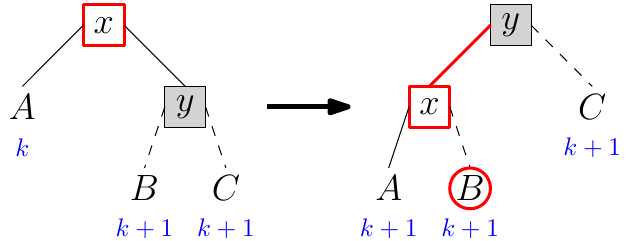
\includegraphics[scale=0.5]{dm3fig/fig3.png}
	\captionof{figure}{\camlline{repare_noir_gauche}, racine \rouge{}.}
	\label{fig:fig3}
\end{minipage}
%
\hfill
%
\begin{minipage}{0.45\linewidth}
    \centering
	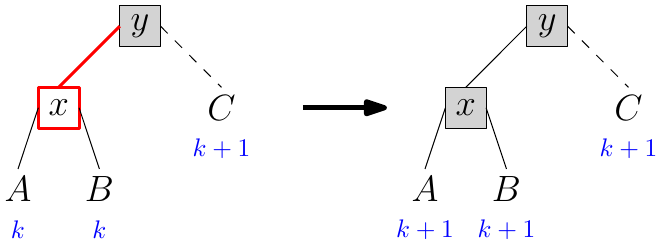
\includegraphics[scale=0.5]{dm3fig/fig4.png}
	\captionof{figure}{\camlline{repare_noir_gauche}, racine noire et fils gauche \rouge{}.}
	\label{fig:fig4}
\end{minipage}

\begin{minipage}{0.45\linewidth}
    \centering
	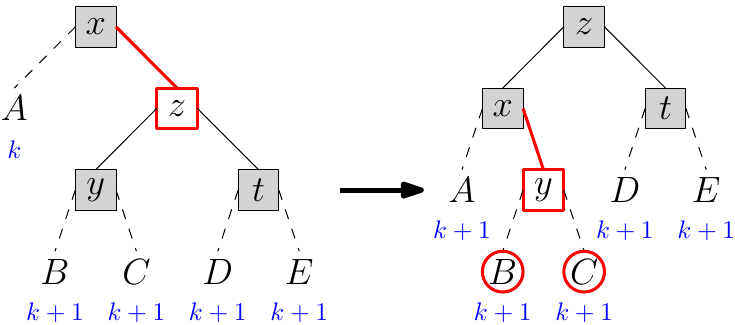
\includegraphics[scale=0.5]{dm3fig/fig6.png}
	\captionof{figure}{\camlline{repare_noir_gauche}, racine noire et fils
droit \rouge{}.}
	\label{fig:fig6}
\end{minipage}
%
\hfill
%
\begin{minipage}{0.45\linewidth}
    \centering
	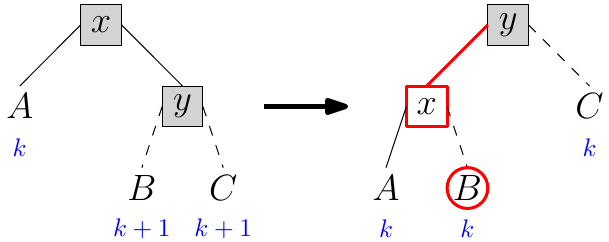
\includegraphics[scale=0.5]{dm3fig/fig5.png}
	\captionof{figure}{\camlline{repare_noir_gauche}, racine noire, deux fils noirs.}
	\label{fig:fig5}
\end{minipage}

\begin{enumerate}[resume]
    \item Quelle est la signification des cercles \rouges{} présent autour de certains nœuds dans les situations finales ?
    
    \boxans{
        Il s'agit de nœuds potentiellement \rouges{} avant le ré-équilibrage, et qui sont maintenant fils d'un autre nœud \rouge{}. Il faut donc potentiellement les changer de couleur.
    }
    
    \item Justifier que tous les cas sont présents, et bien traités.
    
    \boxans{
        \begin{enumerate}
            \itb Si la racine est \rouge{}, alors le fils gauche ne peut pas être \rouge{}. Comme il y a une différence de profondeur noire, alors forcément le fils droit n'est pas vide et est noir. C'est la figure \ref{fig:fig3}.
            
            \itb Si la racine est noire, alors les deux fils ne peuvent pas être tous les deux \rouges{}, car sinon on n'aurait pas de différence de profondeur noire. On a donc soit un fils \rouge{} à gauche (figure \ref{fig:fig4}), soit un fils \rouge{} à droite (figure \ref{fig:fig5}), soit deux fils noirs (figure \ref{fig:fig6}).
            
            \itb Tous les cas sont donc bien présents. On remarque par ailleurs que les arbres obtenus en sortie sont tous des arbres \rouge{}-noir \textbf{corrects} donc tous les cas sont bien traités.
        \end{enumerate}
    }
    
    \item Écrire une fonction \camlline{repare_noir_gauche : ('a rn * bool) -> ('a rn * bool)} dont la spécification est la suivante :
    %
    \begin{enumerate}
        \itt \textbf{Entrée :} un arbre $t$ et un booléen $b$ tels que :
            \begin{enumerate}
                \itstar si $b$ est faux, alors $t$ est un sous-arbre \rouge{}-noir \textbf{correct} ;
                
                \itstar si $b$ est vrai, alors $t$ est de la forme $(g, x, d)$ (la racine de $t$ pouvant être \rouge{} ou noire), $g$ et $d$ sont deux sous-arbres \rouge{}-noir \textbf{corrects}, et la hauteur noire de $d$ vaut exactement un de plus que celle de $g$ ;
            \end{enumerate}
        
        \itt \textbf{Sortie :} un arbre $t'$ et un booléen $b'$ tels que :
            \begin{enumerate}
                \itstar $t'$ est un sous-arbre \rouge{}-noir \textbf{presque correct} ;
                
                \itstar $\etiquettes\left(t'\right) = \etiquettes\left(t\right)$ ;
                
                \itstar en notant $h$ la hauteur de $t$ et $h'$ la hauteur de $t'$, on a $\left\lbrace\begin{array}{rl}
                    b' = \text{\camlline{false}} &\text{ssi} \ h' = h  \\
                    b' = \text{\camlline{true}} &\text{ssi} \ h' = h - 1
                \end{array}\right.$ 
            \end{enumerate}
    \end{enumerate}
    
    \newpage
    
    \begin{ocaml}
let rendre_noir (t : 'a rn) : 'a rn = match t with
    | R(g, x, d) -> N(g, x, d)
    | _ -> t
;;

let repare_noir_gauche ((t, b) : 'a rn * bool) : ('a rn * bool) =
    if not b then (t, false) else match t with
    | R(a, x, N(b, y, c)) | N(a, x, N(b, y, c))
     -> (N(R(a, x, rendre_noir b), y, c), false)
    | N(R(a, x, b), y, c)
     -> (N(N(a, x, b), y, c), false)
    | N(a, x, R(N(b, y, c), z, N(d, t, e))) ->
     (N(N(a, x, R(rendre_noir b, y, rendre_noir c)),z, N(d, t, e)), false)
    | _ -> (t, true)
;;
    \end{ocaml}
    
    \item Compléter la fonction \camlline{supprime_min}.
    
    \begin{ocaml}
let rec supprime_min (arbre : 'a rn) : ('a rn * bool) =
match arbre with
    | V -> failwith "vide"
    | R (V, x, d) -> (V, false)
    | N (V, x, d) -> (d, true)
    | R (g, x, d) | N (g, x, d) -> repare_noir_gauche (supprime_min g)
;;
    \end{ocaml}
        
\end{enumerate}

\subsection{Suppression d'un élément quelconque}

Quand on supprime un élément quelconque, on est amené à traiter le cas d’un arbre dont le fils \textbf{droit} possède une hauteur noire inférieure (de une unité) à celle du fils gauche : c’est par exemple le cas si la suppression du successeur a fait diminuer la hauteur du fils droit.

\begin{enumerate}
    \setcounter{enumi}{10}
    
    \item Représenter les cas symétriques de ceux des figures \ref{fig:fig3} à \ref{fig:fig6}.
    
    \boxans{
    On obtient les arbres suivants :\\\text{}\\
    
    \begin{minipage}{0.45\linewidth}
    \centering
	\begin{tikzpicture}[scale=0.8, level 1/.style={sibling distance=50pt}, level 2/.style={sibling distance=25pt}, level 3/.style={sibling distance=13pt}, level distance=25pt]
    \node at (-2,0) [rectangle, fill=white,draw=main9, thick, inner sep=4pt]{$x$}
    child { 
        node[rectangle, fill=black!12,draw, inner sep=4pt]{$y$}
        child [dashed] { node[label={[font=\tiny,text=main1]below:$k+1$}] {$A$} }
        child [dashed] { node[label={[font=\tiny,text=main1]below:$k+1$}] {$B$} }
    }
    child { node[label={[font=\tiny,text=main1]below:$k$}] {$C$} };
    
    \draw[->, thick] (-0.5, -0.8) -- (0.5, -0.8);;
    
    \node at (2,0) [rectangle, fill=black!12,draw, inner sep=4pt]{$y$}
    child [dashed] { node[label={[font=\tiny,text=main1]below:$k + 1$}] {$A$} }
    child [main9, thick] { 
        node[black, rectangle, fill=white, draw=main9, thick, inner sep=4pt]{$x$}
        child [black, dashed, thin] { node[circle, solid, draw=main9, thick, inner sep=1pt, label={[font=\tiny,text=main1]below:$k+1$}] {$B$} }
        child [black, thin] { node[label={[font=\tiny,text=main1]below:$k+1$}] {$C$} }
    };
\end{tikzpicture}
	\captionof{figure}{\camlline{repare_noir_droite}, racine \rouge{}.}
	\label{fig:fig7}
\end{minipage}
%
\hfill
%
\begin{minipage}{0.45\linewidth}
    \centering
	\begin{tikzpicture}[scale=0.8, level 1/.style={sibling distance=50pt}, level 2/.style={sibling distance=25pt}, level 3/.style={sibling distance=13pt}, level distance=25pt]
    \node at (-2,0) [rectangle, fill=black!12,draw, inner sep=4pt]{$y$}
    child [dashed] { node[label={[font=\tiny,text=main1]below:$k + 1$}] {$A$} }
    child [main9, thick] { 
        node[black, rectangle, fill=white, draw=main9, thick, inner sep=4pt]{$x$}
        child [black, thin] { node[label={[font=\tiny,text=main1]below:$k$}] {$B$} }
        child [black, thin] { node[label={[font=\tiny,text=main1]below:$k$}] {$C$} }
    };
    
    \draw[->, thick] (-0.5, -0.8) -- (0.5, -0.8);;
    
    \node at (2,0) [rectangle, fill=black!12,draw, inner sep=4pt]{$y$}
    child [dashed] { node[label={[font=\tiny,text=main1]below:$k + 1$}] {$A$} }
    child { 
        node[black, rectangle, fill=black!12, draw, inner sep=4pt]{$x$}
        child [black, dashed] { node[label={[font=\tiny,text=main1]below:$k+1$}] {$B$} }
        child [black, dashed] { node[label={[font=\tiny,text=main1]below:$k+1$}] {$C$} }
    };
\end{tikzpicture}
	\captionof{figure}{\camlline{repare_noir_droite}, racine noire et fils droit \rouge.}
	\label{fig:fig8}
\end{minipage}

\text{}\\\text{}\\

\begin{minipage}{0.45\linewidth}
    \centering
	\begin{tikzpicture}[level 1/.style={sibling distance=50pt}, level 2/.style={sibling distance=34pt}, level 3/.style={sibling distance=18pt}, level distance=25pt]
    \node at (-2,0) [rectangle, fill=black!12,draw, inner sep=4pt]{$x$}
    child [main9, thick] { 
        node[black, rectangle, fill=white, draw=main9, thick, inner sep=4pt]{$z$}
        child[thin, black] { 
            node[rectangle, fill=black!12,draw, inner sep=4pt]{$y$}
            child [dashed] { node[label={[font=\tiny,text=main1]below:$k+1$}] {$A$} }
            child [dashed] { node[label={[font=\tiny,text=main1]below:$k+1$}] {$B$} }
        }
        child[thin, black] { 
            node[rectangle, fill=black!12,draw, inner sep=4pt]{$t$}
            child [dashed] { node[label={[font=\tiny,text=main1]below:$k+1$}] {$C$} }
            child [dashed] { node[label={[font=\tiny,text=main1]below:$k+1$}] {$D$} }
        }
    }
    child { node[label={[font=\tiny,text=main1]below:$k$}] {$E$} };
    
    \draw[->, thick] (-0.5, -0.8) -- (0.5, -0.8);;
    
    \node at (2,0) [rectangle, fill=black!12,draw, inner sep=4pt]{$z$}
    child [black, thin] { 
        node[black, thin, rectangle, fill=black!12, draw, inner sep=4pt]{$y$}
        child [dashed] { node[label={[font=\tiny,text=main1]below:$k+1$}] {$A$} }
        child [dashed] { node[label={[font=\tiny,text=main1]below:$k+1$}] {$B$} }
    }
    child [black, thin] { 
        node[black, thin, rectangle, fill=black!12, draw, inner sep=4pt]{$x$}
        child [main9, thick] { 
            node[black, rectangle, fill=white, draw=main9, thick, inner sep=4pt]{$t$}
            child [black, dashed, thin] { node[circle, solid, draw=main9, thick, inner sep=1pt, label={[font=\tiny,text=main1]below:$k+1$}] {$C$} }
            child [black, dashed, thin] { node[circle, solid, draw=main9, thick, inner sep=1pt, label={[font=\tiny,text=main1]below:$k+1$}] {$D$} }
        }
        child [dashed] { node[label={[font=\tiny,text=main1]below:$k+1$}] {$E$} }
    };

    \end{tikzpicture}
	\captionof{figure}{\camlline{repare_noir_gauche}, racine noire et fils gauche \rouge{}.}
	\label{fig:fig10}
\end{minipage}
%
\hfill
%
\begin{minipage}{0.45\linewidth}
    \centering
	\begin{tikzpicture}[scale=0.8, level 1/.style={sibling distance=50pt}, level 2/.style={sibling distance=25pt}, level 3/.style={sibling distance=13pt}, level distance=25pt]
    \node at (-2,0) [rectangle, fill=black!12,draw, inner sep=4pt]{$x$}
    child { 
        node[rectangle, fill=black!12,draw, inner sep=4pt]{$y$}
        child [dashed] { node[label={[font=\tiny,text=main1]below:$k+1$}] {$A$} }
        child [dashed] { node[label={[font=\tiny,text=main1]below:$k+1$}] {$B$} }
    }
    child { node[label={[font=\tiny,text=main1]below:$k$}] {$C$} };
    
    \draw[->, thick] (-0.5, -0.8) -- (0.5, -0.8);;
    
    \node at (2,0) [rectangle, fill=black!12,draw, inner sep=4pt]{$y$}
    child [dashed] { node[label={[font=\tiny,text=main1]below:$k + 1$}] {$A$} }
    child [main9, thick] { 
        node[black, rectangle, fill=white, draw=main9, thick, inner sep=4pt]{$x$}
        child [black, dashed, thin] { node[circle, solid, draw=main9, thick, inner sep=1pt, label={[font=\tiny,text=main1]below:$k+1$}] {$B$} }
        child [black, thin] { node[label={[font=\tiny,text=main1]below:$k+1$}] {$C$} }
    };
\end{tikzpicture}
	\captionof{figure}{\camlline{repare_noir_droite}, racine noire, deux fils noirs.}
	\label{fig:fig9}
\end{minipage}
    }
    
    \item En déduire la fonction \camlline{repare_noir_droite : 'a rn -> bool -> ('a rn * bool)}, \guill{symétrique} de la fonction \camlline{repare_noir_gauche}.
    
    \begin{ocaml}
let repare_noir_droite ((t, b) : 'a rn * bool) : ('a rn * bool) =
    if not b then (t, false) else match t with
    | R(N(a, y, b), x, c) | N(N(a, y, b), x, c)
     -> (N(a, y, R(rendre_noir b, x, c)), false)
    | N(a, y, R(b, x, c))
     -> (N(a, y, N(rendre_noir b, x, c)), false)
    | N(R(N(a, y, b), z, N(c, t, d)), x, e) ->
     (N(N(a, y, b), z, N(R(rendre_noir c, t, rendre_noir d), x, E)), false)
    | _ -> (t, true)
;;
    \end{ocaml}
    
    \item Écrire une fonction \camlline{supprime_aux : 'a rn -> 'a -> ('a rn * bool)} qui prend en entrée un sous-arbre \rouge{}-noir \textbf{correct} $t$ et une clé $x$, et renvoie un couple (t', b) tel que :
    %
    \begin{enumerate}
        \itstar $t'$ est un sous-arbre \rouge{}-noir \textbf{correct} ;
                
        \itstar $\etiquettes\left(t'\right) = \etiquettes\left(t\right) \backslash \left\{x\right\}$ ;
                
        \itstar en notant $h$ la hauteur de $t$ et $h'$ la hauteur de $t'$, on a $\left\lbrace\begin{array}{rl}
            b' = \text{\camlline{false}} &\text{ssi} \ h' = h  \\
            b' = \text{\camlline{true}} &\text{ssi} \ h' = h - 1
        \end{array}\right.$ 
    \end{enumerate}
    
    \begin{ocaml}
let rec supprime_aux (t : 'a rn) (x : 'a) : 'a rn * bool = match t with
    | V -> (V, true)
    | N(V, k, f) | R(V, k, f) when k = x -> supprime_min t;
    | N(f, k, _) | R(f, k, _) when k = x -> (f, false)
    | N(g, k, d) | R(g, k, d) -> if k = x then let t', b= supprime_min d in
    (repare_noir_droite (N(g, min_arbre d, t')), b) else if k < x then supprime_aux d else supprime_aux g
;;
    \end{ocaml}
    
    \item Écrire finalement la fonction \camlline{supprime : 'a rn -> 'a -> 'a rn} qui supprime une clé dans un arbre \rouge{}-noir correct, et renvoie un arbre \rouge{}-noir correct.
    
    \begin{ocaml}
let supprime_aux (t : 'a rn) (x : 'a) = 
    rendre_noir (repare_noir_droite (supprime_aux t a))
;;
    \end{ocaml}
\end{enumerate}

\end{document}